\documentclass{article}
\usepackage{fixltx2e}
\usepackage{float}
\usepackage{amsmath}
\newcommand{\degree}{\ensuremath{^\circ}}
\usepackage{graphicx}
\usepackage[margin=1.15in]{geometry}
\usepackage{setspace}
\usepackage{mathpazo}
\usepackage{algorithmic}



\title{Efficient Pricing of Carbon in the EU and its Effect on Consumers}

\author{Michael Lee \\*
The University of Texas at Austin}



\begin{document}
\onehalfspacing
\maketitle{}
A European single market for electricity is modeled to find the optimal portfolio of energy generation technologies in the presence of a carbon tax. The goal is to find the Pareto optimal carbon tax rate such that both carbon emissions and production costs are minimized. Different sources of electricity-- namely coal, natural gas, nuclear, wind, offshore wind, and solar-- are given levelized costs and carbon dioxide emissions ($CO_{2}$) on a per megawatt-hour (MWh) basis. 20,000 energy portfolios, each with different allocations of the respective generation techniques, are generated via a Monte Carlo process and subsequently evaluated by their per MWh cost and emissions. The cost of each generation technology is related to the upfront capital expense, the variable operations and resource costs (O\&M), the amount of $CO_{2}$ it produces and the EU-wide carbon tax rate. This tax-rate is increased until the most cost-efficient portfolio is also the least $CO_{2}$ producing-- thus finding the optimal carbon tax-rate for aligning environmental and economic interests. {\bf Data extracted from this model suggests that this efficient price is around \$80 USD per ton of $CO_{2}$}\*

The effective production price per MWh from the simulation is then compared to the average industrial power price for each of the EU-member states in order to evaluate the effect of an EU-wide carbon tax on end-users. {\bf The optimal portfolio recommended by the simulation, in conjunction with transport via a Pan-European SuperGrid, will be able to supply power at a similar ($\pm 5\%$) price to the current EU 27 average while dramatically reducing greenhouse gas emissions.}  \
*

% Additionally, the current vulnerability of European power to shocks in the supply of natural gas is evaluated and compared to the optimal portfolio suggested by the model. The results show that {\bf current investment in renewable technologies (whether induced by a carbon tax or not) can dramatically mitigate the adverse effects on consumer prices} caused by a Russian-led price increase. \\*

Further research will investigate the optimal location of each power source given transmission losses and spot pricing and availability for requisite resources (e.g. coal, natural gas, average wind speed etc.), as well as the distortionary effects of subsidies in specific nations.

\newpage{}

\topskip0pt
\vspace*{\fill}
A special thanks to Tom Lee (Project Engineer, Shell North America) for all the insight he shared into the subtleties and dynamics of power management.
\vspace*{\fill}


\newpage{}


\section{The Problem with Carbon}
Over the past 100 years the global temperature has risen $1.53\,^{\circ}\mathrm{F}$. However, since ocean temperature tends to rise slower than land, the overall effect is more pronounced for Earth's landmasses. 

\begin{figure}[H]
	\begin{center}
	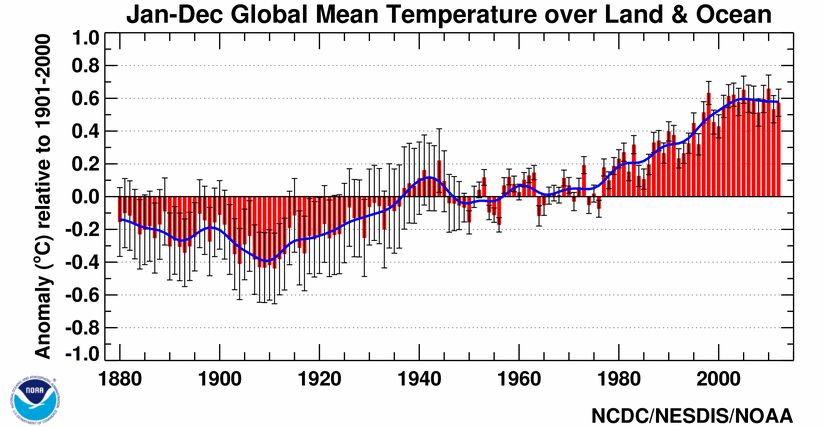
\includegraphics[scale = .5]{Figures/meantemp.png}
	\caption{Rise in Global Temperatures Since 1880 (NOAA, 2011)}
	\end{center}
\end{figure}

While there are those who contest the science, the vast majority of climatologists attribute this sustained rise in global temperatures to the increased use of fossil fuels for transportation and power. In the US, the largest source of these $CO_{2}$ emissions come from the generation of electric power followed by transportation. While no similar data could be found for the EU, Europe's lower car-utilization rate suggests that its percentage of $CO_{2}$ emissions from electric generation is higher than that of the US (global average from electric generation is roughly $\frac{1}{3}$).

\begin{figure}[H]
	\begin{center}
	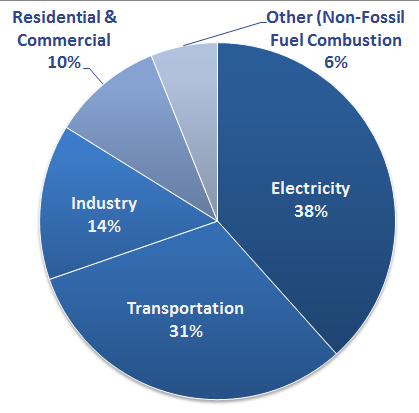
\includegraphics[scale = .5]{Figures/gases-co2.png}
	\caption{Breakdown of Greenhouse Gas Emissions by Source (EPA, 2013)}
	\end{center}
\end{figure}

Clearly, if the EU, and the world, are serious about reducing greenhouse gas emissions, we will have to make changes to the way we generate electric power.

\subsection{Carbon in the EU's Political Landscape}

Currently there is no EU-wide carbon tax. In the 1990's a carbon tax was proposed to the EU Parliament, but this measure failed. However, in 2005 the EU began its emissions trading scheme (EU ETS), commonly referred to as "cap and trade". Under the EU ETS a maximum allowance of greenhouse gases (GHG) is set for each of the 11,000 plants under the regulation. If the operator emits more than its allotted amount of carbon, it is forced to buy carbon permits from other users on the market, thus constraining the aggregate emissions level (European Commission, 2013). \*

Opponents of carbon taxation argue that it is a regressive tax, since it will disproportionally hurt lower-income households. A tax on carbon would cause production costs of electricity to rise, a cost that would ultimately be passed on to the consumer. Assuming all users are charged the same rate for power, the rate increase would represent a larger share of lower-income families income. Additionally, more affluent families are able to afford the upfront capital expenditure associated with buying new, energy efficient appliances, LEED Certified homes, home solar panels, etc. while poorer household will remain reliant on electricity-produced from burning fossil fuels.

\subsubsection{Cap and Trade vs. Carbon Tax}
Theoretically, both the Cap and Trade and a carbon taxation scheme will achieve the same outcome of reducing GHG emissions, however in practice they behave quite differently. 

\begin{figure}[H]
	\begin{center}
	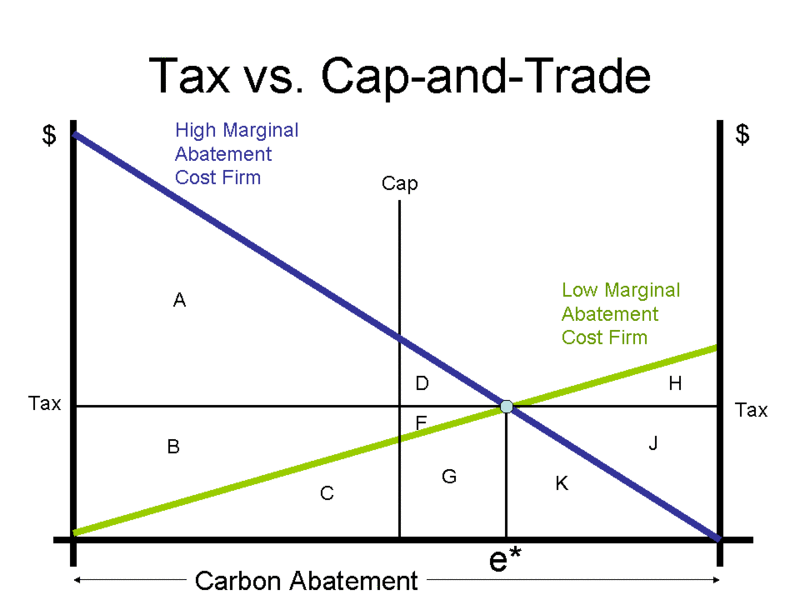
\includegraphics[scale = .4]{Figures/captrade.png}
	\caption{Carbon Tax vs. Cap and Trade (Environmental Economics)}
	\end{center}
\end{figure}


In the EU, all existing power stations were issued a base carbon allowance for free, essentially making the scheme free for them as long as they maintained current emissions levels. On the other hand, a carbon tax will impose immediate costs on all emitters as each unit of carbon has a price. This helps explain why this program was able to pass the ballot while taxation was not (Taschini, 2013). \*

Carbon taxation is more difficult to implement because the price at which it is taxed at is extremely important-- too low and industry might just pay the tax and continue emitting GHG, too high and consumers suffer dramatically higher prices. {\bf It is this pricing problem that this paper centers on.}


\section{Carbon from Electricity}
In addition to being the largest single source of greenhouse gases, electric generation is amongst the low-hanging fruit when it comes to reducing global emissions. Chiefly this is because: 

\begin{itemize}
	\item The scale of power plants means switching one plant from coal to gas will have a large impact
	\item Power plants are designed to last 20+ years, helping capital recovery for a 'green' investment
	\item Technology is already in place for reduced or zero emission sources
	\item Even if personal transports shifts towards electric vehicles, electric generation will need to be cleaner 
\end{itemize}

Electric power demand is predicted to increase in Europe as more and more tasks traditionally fulfilled via internal combustion (IC) or natural gas (e.g. transport and home heating) become electric. This in-and-of itself is good-- large-scale electric generation is much cleaner and energy efficient than IC, however this will force governments and utility companies to build new generation stations. New power plant construction in-turn raises the question of what \emph{type} of power plants should the EU invest in. 

\subsection{The Current State of Power Generation in Europe}
Europe varies greatly when it comes to the methods used to generate electricity. Norway, produces over 90\% of their power from renewable sources, while others such as Malta produce almost 0\% of their power using renewables. Overall, the EU 27 stands at about 18\% generation from renewables. Between 1990 and 2008, the share of electricity produced from renewable sources increased by 288 TWh, an increase of 87.2\% (European Environmental Agency, 2011) 

\begin{figure}[H]
	\begin{center}
	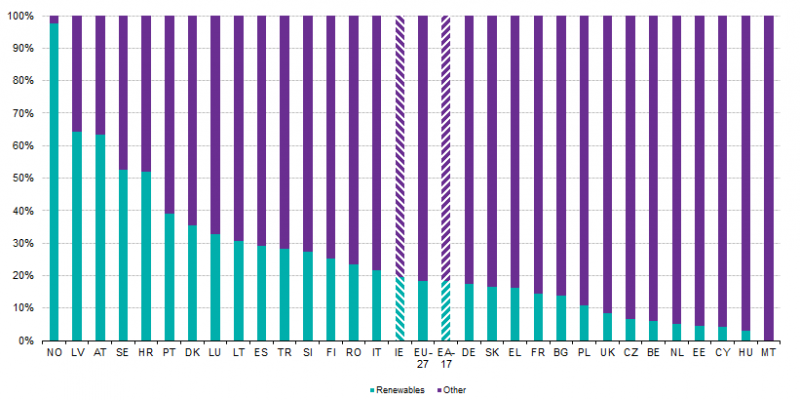
\includegraphics[scale = .6]{Figures/percentrenew.png}
	\caption{Share of Renewables in Electricity Production (Eurostat, 2012)}
	\end{center}
\end{figure}

As seen in {\bf Figure 4} for the vast majority of European nations, electric power is produced primarily by conventional thermal, i.e. burning a fuel to produce heat. Traditionally this has meant coal and oil, but increasingly the world has shifted towards nuclear and natural gas as its main heat sources. As we will see, the various methods of producing this heat have dramatically different environmental impacts. 

\begin{figure}[H]
	\begin{center}
	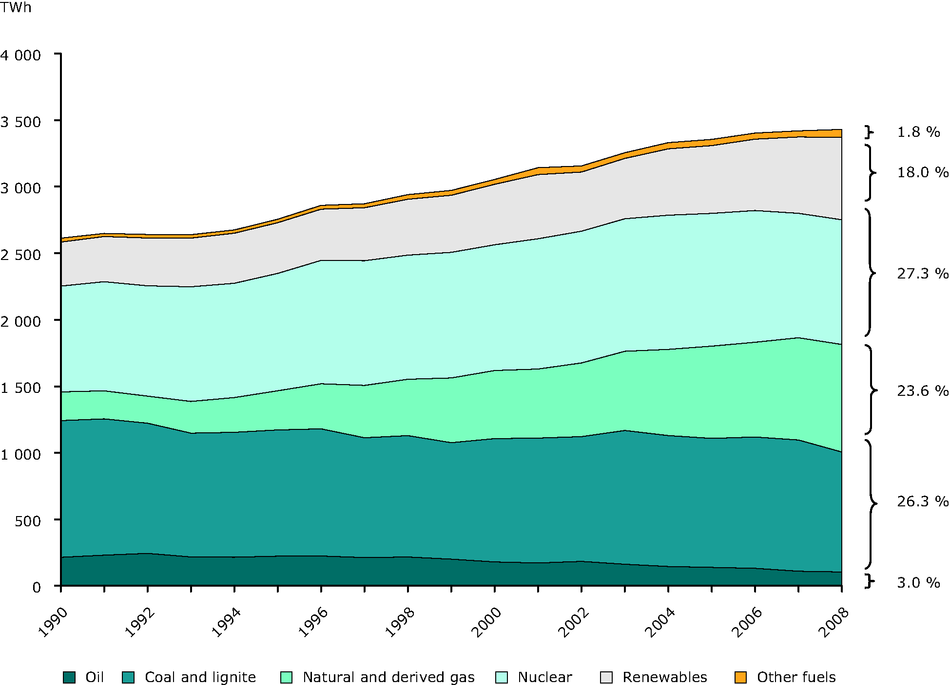
\includegraphics[scale = .5]{Figures/sourceTWh.png}
	\caption{Electric Generation by Fuel Source (Eurostat, 2012)}
	\end{center}
\end{figure}

\subsection{Methods of Generating Electricity}
All types\footnote{With the exception of fuel cells and photovoltaic which rely directly to the flow of electrons} electric generation are derived from the same fundamental principle: Faraday's Law. Faraday’s Law states that a voltage is induced by a change in the magnetic environment of a coil. Electric generators operate on this principle: 1) magnets are placed along a rotating shaft 2) this shaft is placed inside to a coil of wires 3) the shaft is connected to a source of rotary motion (turbine, engine, etc.) 4) the spinning of the shaft causes a change in the magnetic field and 5) an electric voltage is produced. Fossil fuels enter the equation to provide the rotary motion. In the most general sense, some heat source (usually combustion) causes a pressure increase in steam which in turn causes a fan blade to spin. Renewable sources sidestep the combustion process and, in the case of hydroelectric and wind, use the fluid flow to turn the fan blade, or the thermal energy of the sun to heat water as in the case of solar thermal\footnote{It is important to make the distinction between solar thermal and solar photovoltaic. The former uses solar radiation to heat a working fluid while the later exploits a property of certain materials that causes them to shift polarity when heated}\*

As mentioned earlier, the type of fuel used as the heat source dramatically effects the output of $CO_2$ and other pollutants ($NO_x$) per MWh. Renewable sources produce zero GHG emissions, while coal and natural gas produce $CO_2$ as a byproduct of combustion. The relative emissions are shown below:

\begin{figure}[H]
	\begin{center}
	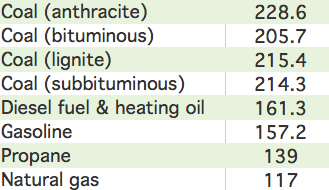
\includegraphics[scale = .75]{Figures/co2fuel.png}
	\caption{Pounds of CO2 Emitted per Million BTU (US Energy Information Administration, 2013)}
	\end{center}
\end{figure}

As seen above, natural gas produces about 57\% less $CO_2$ than bituminous coal (the most commonly used for electricity generation). Thus, it follows that replacing all existing coal power plants with natural gas would reduce GHG emissions by over half! \*

Perhaps a more striking difference than the relative $CO_2$ emissions is the cost difference between sources. When discussing the cost per MWh, we must first establish the different factors internal to the pricing:

\begin{itemize}
\item Capital costs 
\item Fixed operations and management 
\item Variable operations and management (fuel)
\item Transmission investment
\item Capacity factor
\end{itemize}

The first four costs are self-explanatory, but the last is a bit subtle. The capacity factor\footnote{Readers familiar with electro-mechanics will recognize this as the duty cycle} (CF) is the percent of time that the source will run-- a measure of intermittence. For example, if a 1 MW turbine produced 3000h MW over the course of a year, it would have a capacity factor of 34\%. Thus, a 100 MW solar installment (CF=.25) could not reliably provide as much power as a 100 MW gas turbine (CF=.87). 
More formally:

\begin{equation}
Capacity \: Factor = \frac{Actual \: Produced}{Nominal \: Capacity}
\end{equation}

Capacity factors have large implications on the optimal energy portfolio since a certain base load of power will be needed at all times. This suggests that a global optima of cost and emissions exists since a grid comprised completely of renewables would require a nominal capacity of three times the actual requirement-- a three-fold cost increase. {\bf This paper aims to find the Pareto optimal combination of cheap, reliable, polluting thermals with expensive, intermittent, and clean renewables. }\*

Another important distinction is that between \emph{Dispatchable} and \emph{Non-Dispatchable}. Dispatchable technologies are those that can be switched on and off, as well as being able to ramp up or down production based on demand. Dispatchable technologies are more valuable to grid operators because they allow them the flexibility to meet the variable loads demanded throughout the day.\footnote{While technically coal and nuclear are dispatchable, they are more traditionally used to supply base loads since they take more time (days) to ramp up. Aero-derivative gas turbines are the ultimate dispatchable because their production can be started and stopped in a matter of hours.}

\begin{figure}[H]
	\begin{center}
	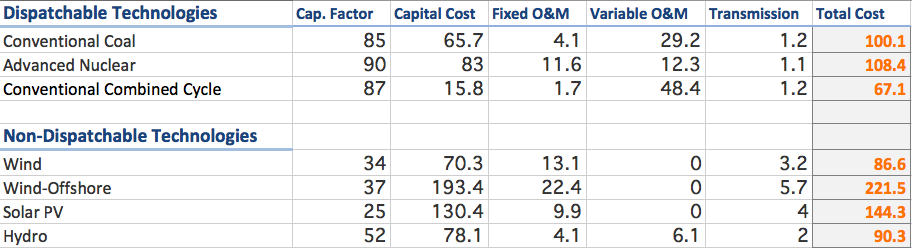
\includegraphics[scale = .5]{Figures/costssource.png}
	\caption{Levelized Costs For Various Generation Technologies (US Energy Information Administration, 2013)}
	\end{center}
\end{figure}


\subsection{Grid Considerations}
The intermittent supply of solar and wind power raises concerns about the stability of the grid. This intermittency, coupled with the unequal demand, could cause blackouts if supply was at a low while demand was at a high (around 4pm). Conversely, if there is not enough demand to meet the supply, blackouts could be caused by wind turbines overloading the transmission lines. Transmission lines, like highways, are limited by their capacity, and large surges of energy can cause them to overload and shutdown, which can potentially cause nationwide voltage drop and subsequent blackout (Cardwell, 2013).   

\begin{figure}[H]
	\begin{center}
	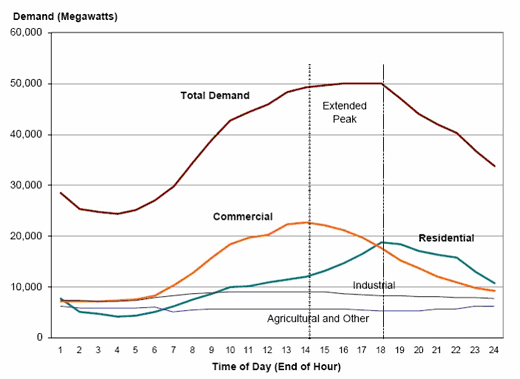
\includegraphics[scale = .75]{Figures/elec_load_demand.png}
	\caption{A Typical Load Profile (Lawrence Berkeley National Laboratory, 2005)}
	\end{center}
\end{figure}


A typical grid operator will want a base load, supplied by nuclear, coal, or natural gas, of around 50\% of peak demand. This way, when the wind blows or the sun shines; there is still a demand node for the generated power to go to. However, since these renewable sources are intermittent, utility companies specify a certain percentage of dispatchable reserves (DR), which can be turned on, should there not be adequate renewable generation to satisfy demand. Gas turbine engines ordinarily generate these reserves. Usually, this reserve ratio is around 70\%. 

\begin{equation}
	DR = Percent\: Generated\: from\: Renewables * Reserve\: Ratio
\end{equation}

Once again, we will see how the intermittent nature of renewable generation technologies effects the optimal energy portfolio as the cost of building a wind or solar installation must also include a the cost of a fractional dispatchable installation.

\subsubsection{European Super Grid}
One of the proposed methods for avoiding the variability of wind and solar resources-- other than using conventional dispatchable reserves-- is to have a more integrated grid, where power could be transported anywhere in Europe for reasonable electrical losses. This would help smooth out the variability of wind speeds in a specific region\footnote{Often cited as "its always windy somewhere"}. The main obstacle to this is the construction of new high voltage direct current (HVDC) lines across the continent. However, this could conceivably be achieved in a decade (Claverton, 2009)

\section{Computational Model}

To evaluate the efficacy of the carbon tax on the utilization rates of multiple generation technologies, a computation model was created. The model uses a Monte Carlo process in conjunction with a statistical tool known as the Dirichlet distribution to randomly create an array of portfolios, each with a different share of the various generation technologies. These energy portfolios were then evaluated based on their cost and $CO_2$ emissions. Certain thresholds were placed on all portfolios to ensure that they were plausible in the real world, namely that a percentage of power was generated from dispatchables (\S2.3). 

\subsection{Monte Carlo Simulation}
Monte Carlo simulations are often used in modeling in situations where a closed-form analytic solution is not readily available or exceedingly computationally intensive. A Monte Carlo simulation relies on repeated random sampling of input variables to obtain an optimal result. In the case of portfolio management (whether it be energy or equities), by randomly choosing the asset allocation percentages and calculating the costs repeatedly, the law of averages states that as the number of simulations approaches infinity, an optimal solution will be found. \*

\subsection{ Dirichlet Distribution}
In the proposed model, sampling was done according to the Dirichlet distribution, which ensures that some number of points in a set, \emph{n}, are randomly sampled such that their sum is equal to some specified total. Thus, the Dirichlet distribution has the statistically appealing property of being the conjugate prior to the parameters of the multinomial distribution. In the computational model, the distribution generates \emph{N} values, bounded by [0,1] that sum to unity. 

\begin{equation}
	p({\bf p}) = Dirichlet ({\bf p, u}) = \frac{1}{Z({\bf u})} \Pi p_{i}^{u_{i}-1}
\end{equation}

\subsection{Dispatchable Reserve Rate}
As mentioned in \S{2.2}, grid operators maintain a reserve of dispatchable capactiy based on the fraction of total capacity generated from renewables. Since this is an \emph{a posteriori} calculation after the desired supply from renewables has been decided, it is calculated in the same manner in the model. \*

The Dirichlet distribution first creates a portfolio consisting of the generation technologies listed in {\bf Figure 7}\footnote{Coal, Nuclear, Natural Gas, Wind, Offshore Wind, Solar, and Hydroelectric} where the sum of the weights equals 1. Afterwards, an algorithm adds the requisite percentage of dispatchable reserves to the portfolio.\footnote{This means that the nominal capacity of the grid is always greater than 100\% supply} For reserve requirement $\lambda$: \\*\\*

\begin{algorithmic}
\FOR{i in portfolio}
\STATE $Portfolio_{Dispatchable \: Reserve}^i = \lambda(Portfolio_{Wind} + Portfolio_{OffshoreWind} + Portfolio_{Solar})$
\ENDFOR
\end{algorithmic}

\subsection{Qualification Criteria}
Over 20,000 portfolios were generated and stored in a matrix. However, many of these did not meet certain the base load requirement, and were removed. With the remaining portfolios, matrix operations were performed 
to calculate the cost and emissions. The portfolios that had the highest and lowest cost and $CO_2$ emissions were then kept for each tax rate.

\subsubsection{Base Load}
If energy portfolios did not meet a predefined percentage of power generation from dispatchables ($\rho$), they were culled from the dataset. 
\begin{algorithmic}
	\IF{$w_{coal} + w_{gas} + w_{nuclear} < \rho$}
		\STATE $delete \: portfolio$
	\ELSE
		\STATE $keep \: portfolio$
	\ENDIF
\end{algorithmic}

All subsequent qualifications (cost and emissions) are done to include the addition of dispatchable reserves to the portfolio.

\subsubsection{Hydroelectric Power}
Since the amount of power generated from hydroelectric sources is fixed by the number of damable rivers, a limit is placed on the percentage of power that can come from such sources. Research shows that this limit is around 15\% of total electric demand. 

\begin{algorithmic}
	\IF{$w_{hydro} < 15\%$}
		\STATE $delete \: portfolio$
	\ELSE
		\STATE $keep \: portfolio$
	\ENDIF
\end{algorithmic}

\subsubsection{Emissions}
Emissions for each portfolio were calculated by using the weighted average of each generation technology and its respective $CO_2$ emissions (as described in {\bf Figure 7}). Where $\epsilon_{i} $ is the $CO_2$ emissions per MWh of generation technology \emph{i}, $w^{ portfolio_n}_{i}$ is the weight of generation technology \emph{i} in $ portfolio_n$, and $CO_{2}^{portfolio_n}$ is the total $CO_2$ emissions for portfolio \emph{n} per MWh. 

\begin{equation}
CO_{2}^{portfolio_n} = \Sigma\; w^{portfolio_n}_{i}* \epsilon_{i} 
\end{equation}

\subsubsection{Costs}
The costs of each portfolio are tied to the rate at which carbon is taxed and the levelized cost per MWh of each generation technology. Thus, if the portfolio produced more carbon, it would cost more than one that produces less \emph{ceteris parabus} This is stated mathematically as:

\begin{equation}
cost^n = w^{n}_{i} * cost_{i} + (\tau*CO{2}^n)
\end{equation}

Where $cost^n$ is the cost of portfolio \emph{n} and $\tau$ is the effective carbon tax rate per tonne of $CO_2$. \*

The tax rate $\tau$ was systematically increased and cost recalculated for the same 20,000 portfolios until {\bf the portfolio with the minimum cost was the portfolio that had the lowest emissions.} This tax rate represents the socially optimal tax rate of \S{1.1.1}.

\section{Results}
The model yielded a final result that matches well with our intuition of what an 'optimal' energy portfolio would look like: nuclear in the place of coal, a diverse mix of renewables, especially hydroelectric\footnote{Hydroelectric is highly represented because it is has a relatively high capacity factor and is semi-dispatchable. While the maximum output is limited by the flux of water, it can be adjusted down from this maximum by gearing the connection between fan and generator shaft.}, and supplemental gas turbines for peak demand. \*

It is my belief that wind power is underrepresented in this model because of its intermittency. If a power grid similar to that explained in \S{2.3.1} is implemented, the capacity factor of wind on a super national level could theoretically be as high as 80\% (Airtricity, 2013)\footnote{The Airtricity proposal is heavily weighted towards offshore wind generation which bypasses some of the NIMBY-ism that plagues wind turbine construction}. If the model takes into account this new capacity factor, wind would surely be the dominant resource in the portfolio, as suggested by Gregor Czish in his study of the Supergrid (Claverton Energy, 2009)\*

It is also important to note that these allocations provided do not take into consideration factors such as geopolitical risk of relying on an extra-national energy supply. The study is also run assuming free market conditions with no government subsidies for nor investment price floors for generated power\footnote{Definitely not the case for the EU. In the UK the government has guaranteed that power generated from renewable sources a price of 87 PS per MW, compared to the market price of around 47 PS}. Perhaps most importantly, the model does not take into consideration the \emph{existing energy mix} of the EU. Thus, the relative cost of building new nuclear plants would be higher than using the existing gas turbines and simply paying the tax. {\bf In this regard, the model is to be seen as a target for an optimal energy mix of the EU as a whole, not as a blueprint for bolt-on construction. }

\subsection{Optimal Carbon Pricing}
The optimal carbon price is defined as the tax rate at which the cost of of producing carbon is equal to the price of using a renewable source. Thus, the optimal carbon tax rate ($\tau$) is found when the portfolio with the lowest cost first becomes the same as the portfolio with the lowest emissions. {\bf By this definition, the optimal tax rate is \$80 USD per ton of carbon.} Past \$80, there is a deadweight loss as no more social benefits are produced in the form of cleaner air yet the cost of production-- and therefor consumer prices-- increases. 

\begin{figure}[H]
	\begin{center}
	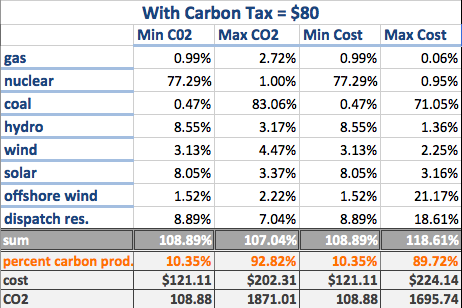
\includegraphics[scale = .6]{Figures/opttax.png}
	\caption{The Optimal Carbon Tax Rate}
	\end{center}
\end{figure}

As seen above, the optimal mixture is heavily weighted towards nuclear and hydroelectric power. Confirming out intuition of what would constitute a 'dirty' portfolio, the most polluting portfolio uses coal as its primary energy source (83\%). In the spirit of the taxation, at a tax rate \$80, the most expensive portfolio is also heavily weighted towards coal (71\%).


\subsection{The Effect of Renewables on Consumer Utility Prices}
For measures such as the European Supergrid to pass, ultimately the voters will have to approve measures that will raise their taxes. In today's economic climate this will prove difficult, it not impossible, unless consumers can be shown that they will benefit in the medium to long term in the form of lower utility prices. Currently, the average price for electricity in the industrial sector\footnote{Industry was used instead of household since it more closely follows the cost of electric production for utility companies. Since the data modeled is based on \emph{production}, this was deemed prudent.} in the nations studied is around 97 Euros per MWh (Europe's Energy Portal, 2013). Converted to US dollars at current exchange rates, this price is around \$132 per MWh. \*

Including an average profit margin for utility providers of 3\% (Yahoo! Finance, 2013), the cost of the portfolio suggested by this model is \$125 per MWh. With a margin of error of plus or minus 5\%, these results imply that a Europe with reduced emissions can be achieve at a similar, if not lower, price than currently facing households. The data produced by this model is confirmed by the research of Gregor Czish (Claverton Energy, 2009) If cleaner air won't motivate consumers, surely this will. 


\section{Future Improvements}
This model will be expanded in the future to consider the location of the power plants suggested by this model. Population dynamic considerations such as population density and population growth will motivate the location of power plants, as will physical factors such as line losses from HVDC transport and local distributive capacity. \*

The future model will also take into consideration the existing mixture of energy resources currently in place in Europe to provide a guideline for which type of power generation the EU should invest in-- and in which order-- to achieve maximum reduction in emissions at the minimum cost. 





% \subsection{Allocation and Europe's Vulnerabilities to Adverse Supply Shocks}
\newpage

\begin{thebibliography}{20}

\bibitem{CO2_Emissions} EIA. "How Much Carbon Dioxide (CO2) Is Produced hen Different Fuels Are Burned?"" \emph{U.S Energy Information Administration}. U.S Energy Information Administration, n.d. Web. 9 Dec.2013.

\bibitem{TaxGraph} Habb, Tim, and John Whitehead. "Econ 101: Carbon Tax vs. Cap-and-Trade." \emph{Environmental Economics}. N.p., n.d. Web. 9 Dec. 2013. 

\bibitem{CapTrade_v_Tax} Tashini, Luca, Simon Dietz, and Naomi Hicks. "Carbon Tax v Cap-and-Trade: Which Is Better?" \emph{The Guardian}. N.p., n.d. Web. 9 Dec. 2013. 

\bibitem{ETS} European Commission. "The EU Emissions Trading System." \emph{Europa}. European Commission, n.d. Web. 9 Dec. 2013. 

\bibitem{PBS} PBS. "Sources of World's CO2 Emissions." \emph{Frontline}. Public Broadcasting Station, n.d. Web. 9 Dec. 2013. 

\bibitem{CO2_Breakdown} EPA. "Overview of Greenhouse Gasses." \emph{EPA}. United States Environmental Protection Agecy, n.d. Web. 9 Dec. 2013. 

\bibitem{Temps} UCAR. "How Much Has the Global Temperature Risen in the Last 100 Years?" \emph{University Corporation for Atmospheric Research}. UCAR, n.d. Web. 9 Dec. 2013. 

\bibitem{MaxRenew} Plumer, Brad. "What Happens if You Add Lots of Wind and Solar Power to the  Grid?" \emph{The Washington Post}. The Washington Post, n.d. Web. 9 Dec. 2013.

\bibitem{Wind} Wind Energy Center. "Wind Power: Capacity Factor, Intermittency, and What Happens When the Wind Doesn't Blow?" \emph{Wind Energy Center}. University of Massachusetts Amherst, n.d. Web. 9 Dec. 2013.  

\bibitem{Grid} Puka, Lidi, and Kacper Szuleki. "Plans to Create a Pan-European Electricity Grid as Part of the Common Energy Market Face a Number of Challenges Before They Can be Realised." \emph{London School of Economics}. LSE, n.d. Web. 9 Dec. 2013. 

\bibitem{Claverton} Andrws, Dave. "Why Do We Need The Supergrid, What Is Its Scope And What Will It Achieve?" \emph{Claverton Energy}. Claverton Energy, 9 June 2009. Web. 9 Dec. 2013. 




\end{thebibliography}

\end{document}



